\documentclass[tikz, border=10pt]{standalone}
\usepackage{tikz}
\usepackage{amsmath}
\usepackage{xcolor}
\usetikzlibrary{arrows.meta, shapes.geometric, positioning, fit,
                decorations.pathmorphing, calc, matrix}

\definecolor{sampleBlue}{HTML}{1565c0}
\definecolor{errorRed}{HTML}{c62828}
\definecolor{correctOrange}{HTML}{e65100}
\definecolor{blockGray}{HTML}{546e7a}
\definecolor{mathBg}{HTML}{f5f5f5}

\tikzset{
  fblock/.style={
    draw=blockGray, fill=blockGray!10, thick,
    rectangle, rounded corners=4pt,
    minimum width=3.2cm, minimum height=1.0cm,
    font=\sffamily\footnotesize, text=blockGray, align=center
  }
}

\begin{document}
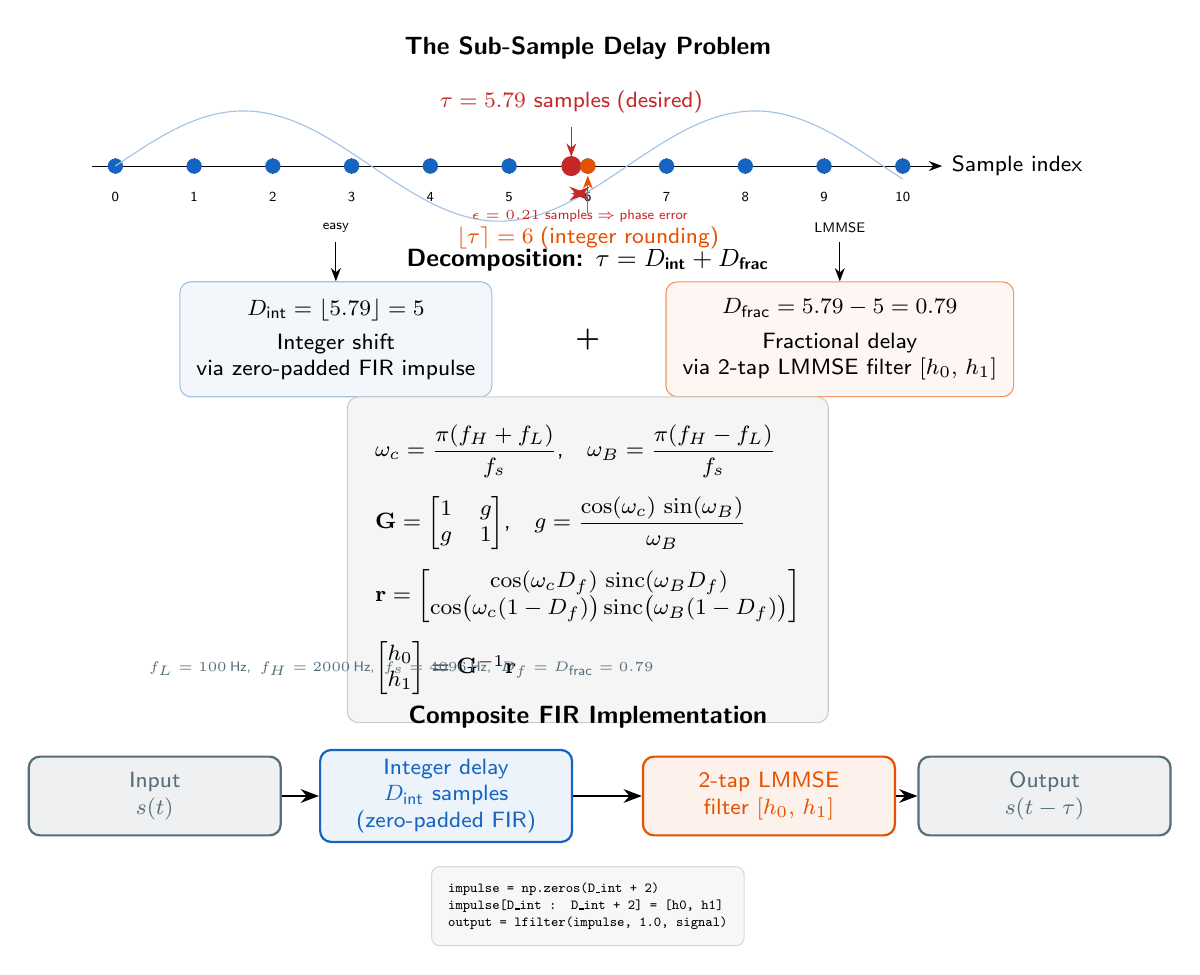
\begin{tikzpicture}[>=Stealth, font=\sffamily\small]

%% ════════════════════════════════════════════════════════════════════
%%  ROW 1 — Problem statement
%% ════════════════════════════════════════════════════════════════════
\node[font=\sffamily\small\bfseries] at (6, 11.5)
    {The Sub-Sample Delay Problem};

% Sample index axis
\draw[->, thin] (-0.3, 10.0) -- (10.5, 10.0)
    node[right, font=\sffamily\footnotesize] {Sample index};

% Integer sample ticks + dots
\foreach \i in {0,1,...,10}{
    \draw[thin] (\i, 9.9) -- (\i, 10.1);
    \filldraw[sampleBlue] (\i, 10.0) circle (0.09);
    \node[below=3pt, font=\sffamily\tiny] at (\i, 9.9) {\i};
}

% Sinusoidal curve through the samples (cosmetic)
\draw[sampleBlue!40, thin, smooth, domain=0:10, samples=200]
    plot (\x, {10.0 + 0.7*sin(deg(2*pi*\x/6.5))});

% Desired fractional position τ = 5.79
\filldraw[errorRed] (5.79, 10.0) circle (0.12);
\draw[errorRed, ->, thin] (5.79, 10.5) -- (5.79, 10.12);
\node[errorRed, above, font=\sffamily\footnotesize]
    at (5.79, 10.55) {$\tau = 5.79$ samples\;(desired)};

% Integer rounded position at 6
\filldraw[correctOrange] (6.0, 10.0) circle (0.09);
\draw[correctOrange, ->, thin] (6.0, 9.4) -- (6.0, 9.88);
\node[correctOrange, below, font=\sffamily\footnotesize]
    at (6.0, 9.35) {$\lfloor\tau\rceil = 6$\;(integer rounding)};

% Error arrow
\draw[errorRed, <->, thick]
    (5.79, 9.65) -- (6.0, 9.65)
    node[midway, below=2pt, font=\sffamily\tiny, errorRed]
    {$\epsilon = 0.21$ samples\;$\Rightarrow$\;phase error};

%% ════════════════════════════════════════════════════════════════════
%%  ROW 2 — Decomposition
%% ════════════════════════════════════════════════════════════════════
\node[font=\sffamily\small\bfseries] at (6, 8.8)
    {Decomposition: $\tau = D_{\text{int}} + D_{\text{frac}}$};

\node[draw=sampleBlue!40, fill=sampleBlue!5, rounded corners=4pt,
      inner sep=6pt, font=\sffamily\footnotesize, align=center]
      (intbox) at (2.8, 7.8) {
    $D_{\text{int}} = \lfloor 5.79 \rfloor = 5$\\[3pt]
    Integer shift\\
    via zero-padded FIR impulse
};
\node[draw=correctOrange!60, fill=correctOrange!5, rounded corners=4pt,
      inner sep=6pt, font=\sffamily\footnotesize, align=center]
      (fracbox) at (9.2, 7.8) {
    $D_{\text{frac}} = 5.79 - 5 = 0.79$\\[3pt]
    Fractional delay\\
    via 2-tap LMMSE filter $[h_0,\,h_1]$
};

% Decomposition equation
\node[font=\sffamily\normalsize] at (6.0, 7.8)
    {$\boldsymbol{+}$};
\draw[<-, thin] (intbox.north) -- ++(0, 0.5)
    node[above, font=\sffamily\tiny] {easy};
\draw[<-, thin] (fracbox.north) -- ++(0, 0.5)
    node[above, font=\sffamily\tiny] {LMMSE};

%% ════════════════════════════════════════════════════════════════════
%%  ROW 3 — LMMSE equations
%% ════════════════════════════════════════════════════════════════════
\node[font=\sffamily\small\bfseries] at (6, 6.4)
    {2-tap LMMSE Gram System};

\node[draw=black!20, fill=mathBg, rounded corners=4pt,
      inner sep=10pt, align=left, font=\sffamily\footnotesize]
      (grambox) at (6.0, 5.0) {
    $\omega_c = \dfrac{\pi(f_H + f_L)}{f_s}$,\quad
    $\omega_B = \dfrac{\pi(f_H - f_L)}{f_s}$ \\[6pt]
    $\mathbf{G} =
     \begin{bmatrix} 1 & g \\ g & 1 \end{bmatrix}$,\quad
    $g = \dfrac{\cos(\omega_c)\,\sin(\omega_B)}{\omega_B}$ \\[6pt]
    $\mathbf{r} =
     \begin{bmatrix}
       \cos(\omega_c D_f)\,\operatorname{sinc}(\omega_B D_f) \\
       \cos\!\left(\omega_c(1-D_f)\right)\operatorname{sinc}\!\left(\omega_B(1-D_f)\right)
     \end{bmatrix}$ \\[6pt]
    $\begin{bmatrix}h_0\\h_1\end{bmatrix}
     = \mathbf{G}^{-1}\mathbf{r}$
};

% Parameter values annotation
\node[font=\sffamily\tiny, text=blockGray, anchor=west] at (0.3, 3.6)
    {$f_L = 100\,\text{Hz}$,\;
     $f_H = 2000\,\text{Hz}$,\;
     $f_s = 4096\,\text{Hz}$,\;
     $D_f = D_{\text{frac}} = 0.79$};

%% ════════════════════════════════════════════════════════════════════
%%  ROW 4 — Filter block diagram
%% ════════════════════════════════════════════════════════════════════
\node[font=\sffamily\small\bfseries] at (6, 3.0)
    {Composite FIR Implementation};

\node[fblock] (input) at (0.5, 2.0) {Input\\$s(t)$};

\node[fblock, draw=sampleBlue, fill=sampleBlue!8, text=sampleBlue]
     (intfir) at (4.2, 2.0)
     {Integer delay\\$D_{\text{int}}$ samples\\(zero-padded FIR)};

\node[fblock, draw=correctOrange, fill=correctOrange!8, text=correctOrange]
     (lmmse) at (8.3, 2.0)
     {2-tap LMMSE\\filter $[h_0,\,h_1]$};

\node[fblock] (output) at (11.8, 2.0) {Output\\$s(t-\tau)$};

\draw[->, thick] (input)  -- (intfir);
\draw[->, thick] (intfir) -- (lmmse);
\draw[->, thick] (lmmse)  -- (output);

% Code snippet below
\node[draw=black!15, fill=black!3, rounded corners=3pt,
      inner sep=6pt, font=\ttfamily\tiny, align=left] at (6.0, 0.6) {
    impulse = np.zeros(D\_int + 2)\\
    impulse[D\_int : D\_int + 2] = [h0, h1]\\
    output  = lfilter(impulse, 1.0, signal)
};

\end{tikzpicture}
\end{document}
